\thispagestyle{empty}
\definecolor{Gray}{rgb}{ .949,  .949,  .949}
\newcolumntype{g} {>{\columncolor{Gray}}c}
\chapter{Análisis de Semejantes. Helicóptero Semilla}

Tal y como se ha reflejado en la introducción, el proceso a seguir para optener un diseño preliminar, será el análisis de semejantes.
Este análisis consiste en crear una base de datos de aeronaves ya existentes, cuyas características sean similares a las que podría tener la nuestra, de manera que mediante un análisis estadístico se pueda obtener una primera aproximación de algunas características de nuestra aeronave.\\

\section{Estudio de Aeronaves de Referencia}

Dado que el objetivo es el diseño de un helicóptero no tripulado de 450 Kg de \emph{MTOW}, los vehículos a analizar serán helicópteros de una masa similar, en torno a 400-500 kg, pero al no existir una cantidad suficiente dentro de este margen, se ha decidido ampliar este.
En las tablas \ref{ASomega} y \ref{AS} se encuentran los helicópteros seleccionados para el análisis

%PROBLEMAS CON LAS TABLAS, BUSCAR COMO ARREGLAR EL DESASTRE DE TABLA QUE NO ENTRA, TAL VEZ DIVIDIRLO EN 2 SEA SUFICIENTE
\begin{table}[htbp]
	\centering
	\begin{tabular}{|l|c|c|c|c|c|c|c|}
		\hline
		\rowcolor[rgb]{ .851,  .851,  .851} MODELO & \multicolumn{1}{l|}{MTOW[kg]} & \multicolumn{1}{l|}{d[m]} & \multicolumn{1}{l|}{$\Omega$ [rad/s]} & \multicolumn{1}{l|}{b} & \multicolumn{1}{l|}{$b_a$} & \multicolumn{1}{l|}{$h_{max}$[m]} & \multicolumn{1}{l|}{$V_{max}$[km/h]} \\ \hline
		\rowcolor[rgb]{ .949,  .949,  .949} SA-200 Weasel & \cellcolor[rgb]{ 1,  1,  1}70 & \cellcolor[rgb]{ 1,  1,  1}2,07 & \cellcolor[rgb]{ 1,  1,  1}167,55 & \cellcolor[rgb]{ 1,  1,  1}2 & \cellcolor[rgb]{ 1,  1,  1}6 & \cellcolor[rgb]{ 1,  1,  1}3100 & \cellcolor[rgb]{ 1,  1,  1}167 \\
		\hline
		\rowcolor[rgb]{ .949,  .949,  .949} Yamaha R-50 & \cellcolor[rgb]{ 1,  1,  1}90 & \cellcolor[rgb]{ 1,  1,  1}3,07 & \cellcolor[rgb]{ 1,  1,  1}88,6 & \cellcolor[rgb]{ 1,  1,  1}2 & \cellcolor[rgb]{ 1,  1,  1}2 & \cellcolor[rgb]{ 1,  1,  1}300 & \cellcolor[rgb]{ 1,  1,  1}VACÍO \\
		\hline
		\rowcolor[rgb]{ .949,  .949,  .949} R-350 & \cellcolor[rgb]{ 1,  1,  1}150 & \cellcolor[rgb]{ 1,  1,  1}3,5 & \cellcolor[rgb]{ 1,  1,  1}82,86 & \cellcolor[rgb]{ 1,  1,  1}3 & \cellcolor[rgb]{ 1,  1,  1}2 & \cellcolor[rgb]{ 1,  1,  1}2500 & \cellcolor[rgb]{ 1,  1,  1}120 \\
		\hline
		\rowcolor[rgb]{ .949,  .949,  .949} SD 150 Hero & \cellcolor[rgb]{ 1,  1,  1}150 & \cellcolor[rgb]{ 1,  1,  1}3,5 & \cellcolor[rgb]{ 1,  1,  1}105,14 & \cellcolor[rgb]{ 1,  1,  1}3 & \cellcolor[rgb]{ 1,  1,  1}2 & \cellcolor[rgb]{ 1,  1,  1}4000 & \cellcolor[rgb]{ 1,  1,  1}90 \\
		\hline
		\rowcolor[rgb]{ .949,  .949,  .949} APID 55 & \cellcolor[rgb]{ 1,  1,  1}160 & \cellcolor[rgb]{ 1,  1,  1}3,3 & \cellcolor[rgb]{ 1,  1,  1}54,54 & \cellcolor[rgb]{ 1,  1,  1}2 & \cellcolor[rgb]{ 1,  1,  1}2 & \cellcolor[rgb]{ 1,  1,  1}3000 & \cellcolor[rgb]{ 1,  1,  1}90 \\
		\hline
		\rowcolor[rgb]{ .949,  .949,  .949} APID 60 & \cellcolor[rgb]{ 1,  1,  1}180 & \cellcolor[rgb]{ 1,  1,  1}3,3 & \cellcolor[rgb]{ 1,  1,  1}90,97 & \cellcolor[rgb]{ 1,  1,  1}2 & \cellcolor[rgb]{ 1,  1,  1}2 & \cellcolor[rgb]{ 1,  1,  1}3000 & \cellcolor[rgb]{ 1,  1,  1}110 \\
		\hline
		\rowcolor[rgb]{ .949,  .949,  .949} Camcopter S100 & \cellcolor[rgb]{ 1,  1,  1}200 & \cellcolor[rgb]{ 1,  1,  1}3,4 & \cellcolor[rgb]{ 1,  1,  1}130,73 & \cellcolor[rgb]{ 1,  1,  1}2 & \cellcolor[rgb]{ 1,  1,  1}2 & \cellcolor[rgb]{ 1,  1,  1}5500 & \cellcolor[rgb]{ 1,  1,  1}222 \\
		\hline
		\rowcolor[rgb]{ .949,  .949,  .949} Pelícano & \cellcolor[rgb]{ 1,  1,  1}200 & \cellcolor[rgb]{ 1,  1,  1}3,3 & \cellcolor[rgb]{ 1,  1,  1}81,22 & \cellcolor[rgb]{ 1,  1,  1}2 & \cellcolor[rgb]{ 1,  1,  1}2 & \cellcolor[rgb]{ 1,  1,  1}3600 & \cellcolor[rgb]{ 1,  1,  1}180 \\
		\hline
		\rowcolor[rgb]{ .949,  .949,  .949} DP 5X Wasp & \cellcolor[rgb]{ 1,  1,  1}227 & \cellcolor[rgb]{ 1,  1,  1}3,2 & \cellcolor[rgb]{ 1,  1,  1}127,33 & \cellcolor[rgb]{ 1,  1,  1}4 & \cellcolor[rgb]{ 1,  1,  1}4 & \cellcolor[rgb]{ 1,  1,  1}4100 & \cellcolor[rgb]{ 1,  1,  1}160 \\
		\hline
	\end{tabular}%
	\caption{Valores de diferentes parámetros de las aeronaves empleadas para el análisis de semejantes cuyos valores de velocidad de giro del rotor principal han sido publicados.}
	\label{ASomega}
\end{table}%

\begin{table}[htbp]
	\centering
	\begin{tabular}{|l|c|c|c|c|c|c|}
		\hline
		\rowcolor[rgb]{ .851,  .851,  .851} MODELO & \multicolumn{1}{l|}{MTOW[kg]} & \multicolumn{1}{l|}{d[m]} & \multicolumn{1}{l|}{b} & \multicolumn{1}{l|}{$b_a$} & \multicolumn{1}{l|}{$h_{max}$[m]} & \multicolumn{1}{l|}{$V_{max}$[km/h]} \\
		\hline
		\rowcolor[rgb]{ .949,  .949,  .949} Scout B1-100 & \cellcolor[rgb]{ 1,  1,  1}77 & \cellcolor[rgb]{ 1,  1,  1}3,2 & \cellcolor[rgb]{ 1,  1,  1}2 & \cellcolor[rgb]{ 1,  1,  1}2 & \cellcolor[rgb]{ 1,  1,  1}VACÍO & \cellcolor[rgb]{ 1,  1,  1}VACÍO \\
		\hline
		\rowcolor[rgb]{ .949,  .949,  .949} Neo S300 & \cellcolor[rgb]{ 1,  1,  1}85 & \cellcolor[rgb]{ 1,  1,  1}3 & \cellcolor[rgb]{ 1,  1,  1}3 & \cellcolor[rgb]{ 1,  1,  1}2 & \cellcolor[rgb]{ 1,  1,  1}VACÍO & \cellcolor[rgb]{ 1,  1,  1}VACÍO \\
		\hline
		\rowcolor[rgb]{ .949,  .949,  .949} Skeldar V-200 & \cellcolor[rgb]{ 1,  1,  1}235 & \cellcolor[rgb]{ 1,  1,  1}4,6 & \cellcolor[rgb]{ 1,  1,  1}2 & \cellcolor[rgb]{ 1,  1,  1}2 & \cellcolor[rgb]{ 1,  1,  1}3500 & \cellcolor[rgb]{ 1,  1,  1}140 \\
		\hline
		\rowcolor[rgb]{ .949,  .949,  .949} Tanan EADS & \cellcolor[rgb]{ 1,  1,  1}300 & \cellcolor[rgb]{ 1,  1,  1}5 & \cellcolor[rgb]{ 1,  1,  1}2 & \cellcolor[rgb]{ 1,  1,  1}2 & \cellcolor[rgb]{ 1,  1,  1}4000 & \cellcolor[rgb]{ 1,  1,  1}150 \\
		\hline
		\rowcolor[rgb]{ .949,  .949,  .949} SVU-200 & \cellcolor[rgb]{ 1,  1,  1}360 & \cellcolor[rgb]{ 1,  1,  1}4,92 & \cellcolor[rgb]{ 1,  1,  1}4 & \cellcolor[rgb]{ 1,  1,  1}2 & \cellcolor[rgb]{ 1,  1,  1}4200 & \cellcolor[rgb]{ 1,  1,  1}209 \\
		\hline
		\rowcolor[rgb]{ .949,  .949,  .949} Cicare 7B & \cellcolor[rgb]{ 1,  1,  1}430 & \cellcolor[rgb]{ 1,  1,  1}6,28 & \cellcolor[rgb]{ 1,  1,  1}2 & \cellcolor[rgb]{ 1,  1,  1}2 & \cellcolor[rgb]{ 1,  1,  1}3000 & \cellcolor[rgb]{ 1,  1,  1}194 \\
		\hline
		\rowcolor[rgb]{ .949,  .949,  .949} Robinson R-22 & \cellcolor[rgb]{ 1,  1,  1}622 & \cellcolor[rgb]{ 1,  1,  1}7,67 & \cellcolor[rgb]{ 1,  1,  1}2 & \cellcolor[rgb]{ 1,  1,  1}2 & \cellcolor[rgb]{ 1,  1,  1}4267 & \cellcolor[rgb]{ 1,  1,  1}188 \\
		\hline
		\rowcolor[rgb]{ .949,  .949,  .949} VSR700 & \cellcolor[rgb]{ 1,  1,  1}680 & \cellcolor[rgb]{ 1,  1,  1}7,2 & \cellcolor[rgb]{ 1,  1,  1}3 & \cellcolor[rgb]{ 1,  1,  1}7 & \cellcolor[rgb]{ 1,  1,  1}3600 & \cellcolor[rgb]{ 1,  1,  1}187 \\
		\hline
		\rowcolor[rgb]{ .949,  .949,  .949} Brantly B-2 & \cellcolor[rgb]{ 1,  1,  1}757 & \cellcolor[rgb]{ 1,  1,  1}7,24 & \cellcolor[rgb]{ 1,  1,  1}3 & \cellcolor[rgb]{ 1,  1,  1}2 & \cellcolor[rgb]{ 1,  1,  1}3290 & \cellcolor[rgb]{ 1,  1,  1}161 \\
		\hline
		\rowcolor[rgb]{ .949,  .949,  .949} Schweizer 300 & \cellcolor[rgb]{ 1,  1,  1}930 & \cellcolor[rgb]{ 1,  1,  1}8,2 & \cellcolor[rgb]{ 1,  1,  1}3 & \cellcolor[rgb]{ 1,  1,  1}2 & \cellcolor[rgb]{ 1,  1,  1}4300 & \cellcolor[rgb]{ 1,  1,  1}176 \\
		\hline
	\end{tabular}%
	\caption{Valores de diferentes parámetros de las aeronaves empleadas para el análisis de semejantes cuyos valores de velocidad de giro del rotor principal no han sido publicados.}
	\label{AS}
\end{table}%



Una vez se ha obtenido la selección de aeronaves semejantes, se procede a realizar un análisis estadístico de las distintas características de los mismos para obtener unos primeros valores de diseño. Al ser la característica más definitoria de la aeronave el peso máximo al despegue, se observará la evolución de los distintos parámetros con el MTOW.
En este capítulo se pueden observar las gráficas que se obtienen del análisis anterior para cada parámetro, incluyendo una línea de tendencia que nos permita obtener una primera aproximación en el diseño. Cabe indicar que se han omitido, en las gráficas correspondientes, aquellos vehículos cuyas características no eran conocidas, sin eliminarlos del resto de ellas. Las líneas de tendencia se han generado usando una aproximación lineal, lo cual puede llevar a una mala aproximación dependiendo de los datos.


\begin{figure}
	\centering
	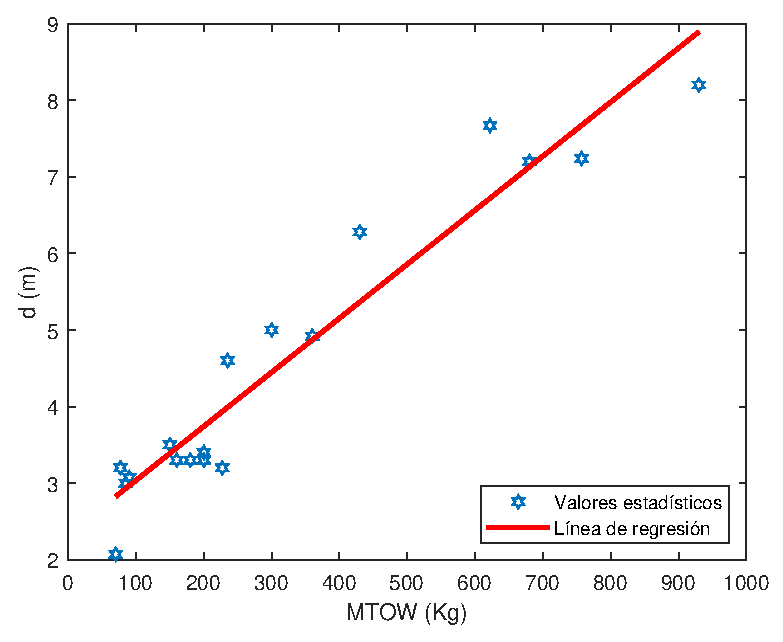
\includegraphics[width=80mm]{graficos/anald}
	\caption{Relación entre los diámetros de las palas de los helicópteros y sus MTOW junto a su línea de tendencia.}
	\label{diamAS}
\end{figure}
\begin{figure}
	\centering
	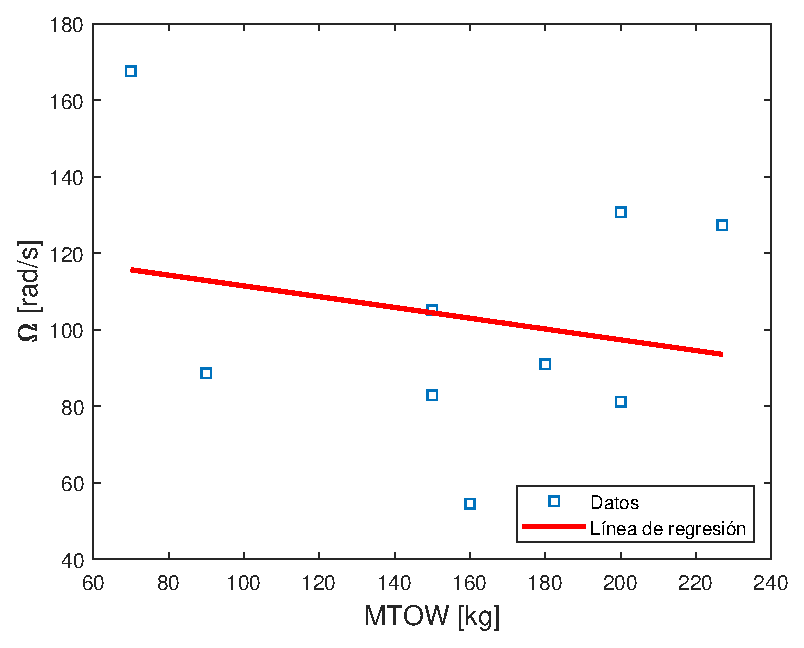
\includegraphics[width=80mm]{graficos/analomega}
	\caption{Relación entre las velocidades de giro del rotor de los helicópteros y sus MTOW junto a su línea de tendencia.}
	\label{omegaAS}
\end{figure}
\begin{figure}
	\centering
	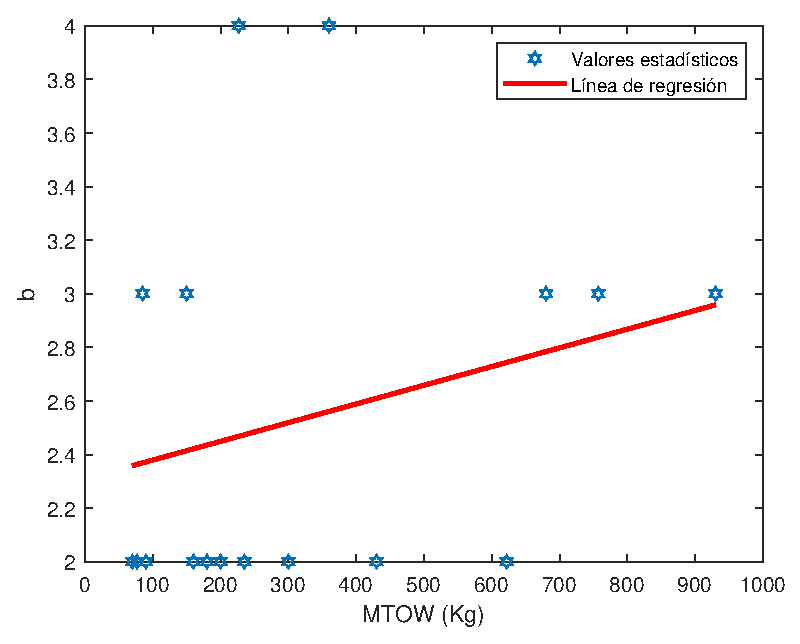
\includegraphics[width=80mm]{graficos/analb}
	\caption{Relación entre el número de palas del rotor principal de los helicópteros y sus MTOW junto a su línea de tendencia.}
	\label{bAS}
\end{figure}
\begin{figure}
	\centering
	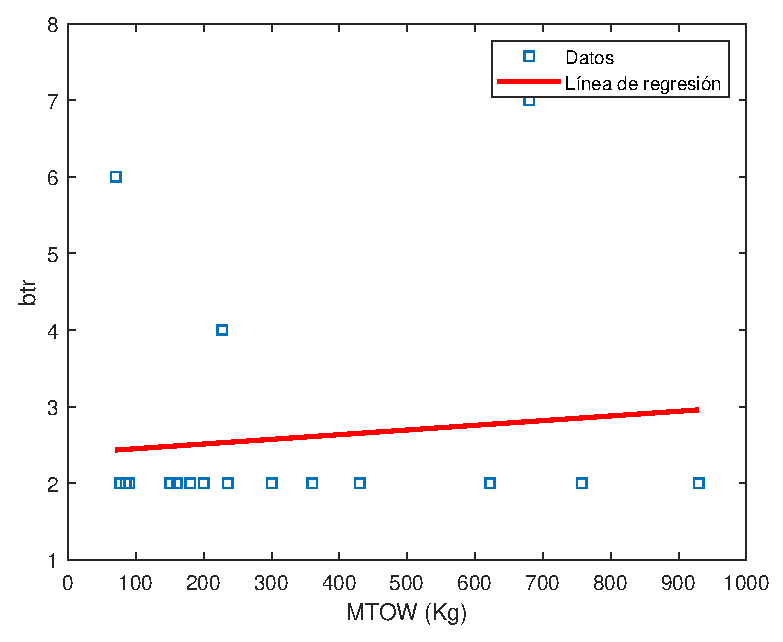
\includegraphics[width=80mm]{graficos/analbtr}
	\caption{Relación entre el número de palas del rotor antipar de los helicópteros y sus MTOW junto a su línea de tendencia.}
	\label{baAS}
\end{figure}
\begin{figure}
	\centering
	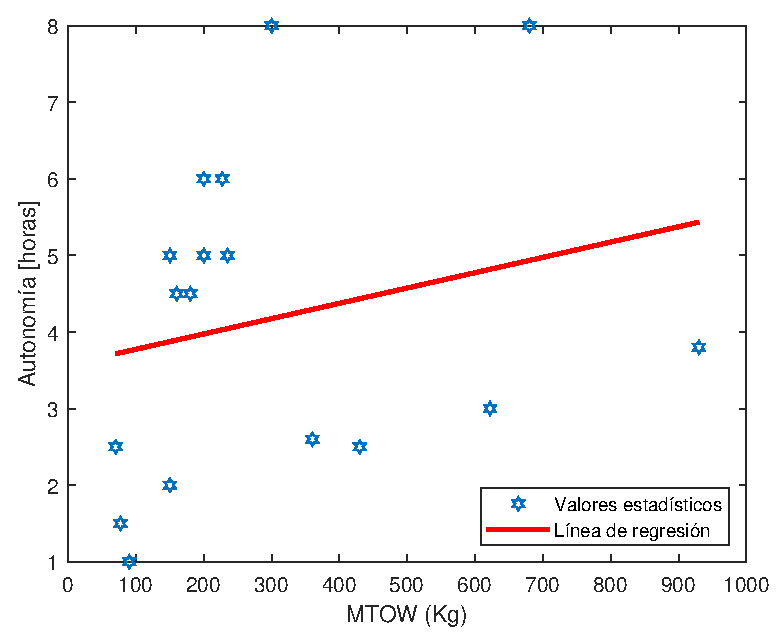
\includegraphics[width=80mm]{graficos/analaut}
	\caption{Relación entre las autonomías de los helicópteros y sus MTOW junto a su línea de tendencia.}
	\label{autAS}
\end{figure}
\begin{figure}
	\centering
	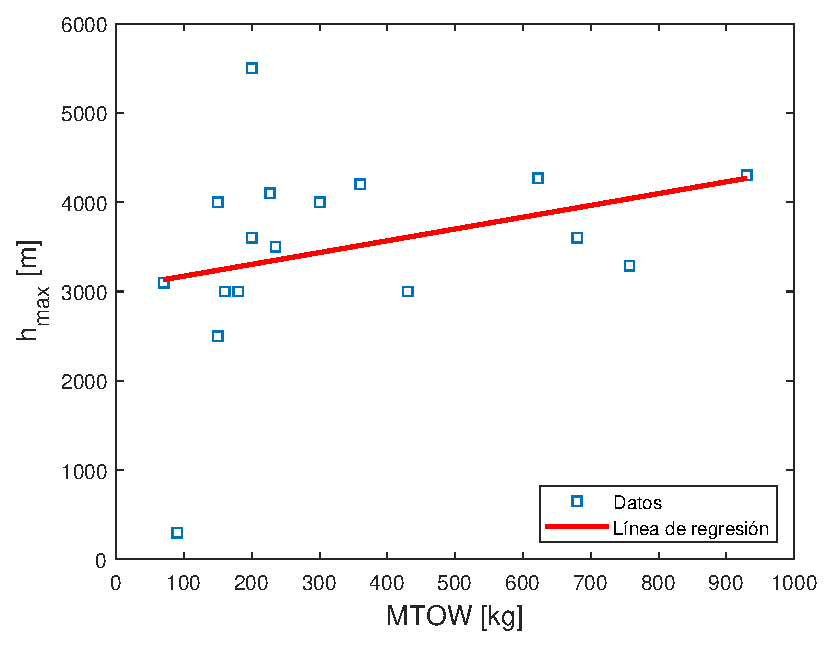
\includegraphics[width=80mm]{graficos/analtecho}
	\caption{Relación entre los techos de vuelo de los helicópteros y sus MTOW junto a su línea de tendencia.}
	\label{techoAS}
\end{figure}
\begin{figure}
	\centering
	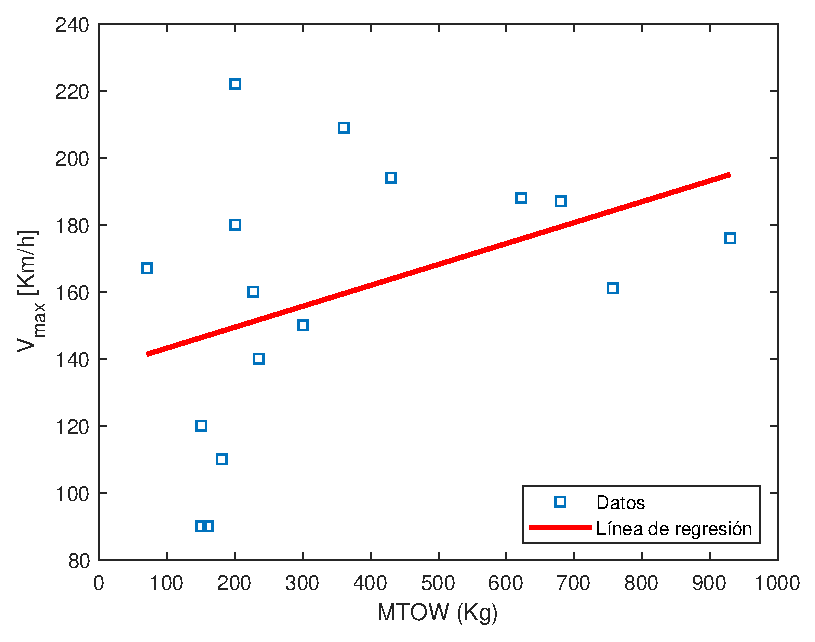
\includegraphics[width=80mm]{graficos/analv}
	\caption{Relación entre las velocidades máximas de avance de los helicópteros y sus MTOW junto a su línea de tendencia.}
	\label{vAS}
\end{figure}

Como se puede observar, muchos helicópteros comparten características aunque sus pesos sean muy distintos, y algunas líneas de tendencia se alejan considerablemente de los valores promedio para la zona que corresponde a 450 kg. Esto se debe principalmente a la falta de datos de referencia, los pocos desarrollos que se han dado de aeronaves de ala rotatoria en el entorno de pesos dado dificultan en gran medida la verificación de nuestro modelo al no existir una norma de diseño en la que basarnos. Los desarrollos han sido dispersos, así que los parámetros iniciales de diseño no se basarán únicamente en los valores de tendencia obtenidos.
 
\begin{itemize}
	\item $d$: 5,5 m
	\item $\Omega$: 120 rad/s
	\item $b$: 2
	\item $b_{a}$ antipar: 2
	\item $t_{e}$: 3 horas
	\item $h_{max}$: 3200 m
	\item $V_{max}$: 190 m/s
\end{itemize}

Queda patente que en algunos casos, se han aproximado los valores omitiendo las líneas de tendencia, usando en su lugar los valores de los helicópteros cuyos MTOW son más próximos al de la aeronave a diseñar.

\section{Descripción Helicóptero Base}

Para poder realizar una simulación en \emph{HEROES} se empleará un helicóptero base que nos ayudará a obtener un modelo preliminar de forma mucho más rápida. Los requisitos de esta aeronave serán que resulte semejante al diseño que se busca, de manera que pueda reescalarse según las necesidades. Para este proyecto se ha escogido el Bölkow Bo 105, un helicóptero utilitario monorrotor, cuyas características se exponen a continuación.

\subsection{Rotor Principal del Bo 105}

Los parámetros necesarios para definir el rotor principal de un helicóptero incluyen datos geométricos, aerodinámicos y de inercia. Los correspondientes al Bo 105 se encuentran recogidos en la tabla \ref{RPBo}.
Para simplificar los cálculos, la pala se modeliza como sólido rígido, unida al rotor por un muelle de constante $k_\beta$.
Además el tensor de inercia de la pala se ha modelizado de la siguiente manera.

\begin{equation}
[I_B]=\left[	
\begin{array}{ccc}
I_\beta & 0 & 0\\
0 & I_\theta & 0\\
0 & 0 & I_\zeta
\end{array}
\right]
\end{equation}

\begin{table}[htbp]
	\centering
	\begin{tabular}{|>{\columncolor{Gray}}c|c|}
		\hline
		\cellcolor{Gray}Radio de las palas ($R$) & \cellcolor[rgb]{ 1,  1,  1}4.91 $m$ \\ \hline
		\cellcolor{Gray}Excentricidad ($e$)& \cellcolor[rgb]{ 1,  1,  1}0 $m$ \\ \hline
		\cellcolor{Gray}Número de palas ($b$) & \cellcolor[rgb]{ 1,  1,  1}4 \\ \hline
		\cellcolor{Gray}Torsión lineal de los perfiles ($\theta_1$) & \cellcolor[rgb]{ 1,  1,  1}-0.14 \\ \hline
		\cellcolor{Gray}Pendiente de la curva de sustentación ($\alpha$) & \cellcolor[rgb]{ 1,  1,  1}6.113 $rad^{-1}$ \\ \hline
		\cellcolor{Gray} & \cellcolor[rgb]{ 1,  1,  1}0.0074 \\ \hhline{|~|-|}
		\cellcolor{Gray} & \cellcolor[rgb]{ 1,  1,  1}0.00961 $rad^{-1}$ \\ \hhline{|~|-|}
		\multirow{-3}{*}{\cellcolor{Gray}Parámetros de la polar ($\delta_0$, $\delta_1$, $\delta_2$)} & \cellcolor[rgb]{ 1,  1,  1}0.29395 $rad^{-2}$ \\ \hline
		\cellcolor{Gray}Velocidad de giro del rotor ($\Omega$) & \cellcolor[rgb]{ 1,  1,  1}44.4 $rad/s$ \\ \hline
		\cellcolor{Gray}Cuerda del perfil ($c$) & \cellcolor[rgb]{ 1,  1,  1}6.113 \\ \hline
		\cellcolor{Gray}Momento de inercia de la pala en batimiento ($I_\beta$) & \cellcolor[rgb]{ 1,  1,  1}231.7 $kgm^2$ \\ \hline
		\cellcolor{Gray}Momento de inercia de la pala en paso ($I_\theta$) & \cellcolor[rgb]{ 1,  1,  1}7 $kgm^2$ \\ \hline
		\cellcolor{Gray}Momento de inercia de la pala en arrastre ($I_\zeta$) & \cellcolor[rgb]{ 1,  1,  1}238.7 $kgm^2$ \\ \hline
		\cellcolor{Gray}Posición del centro de gravedad de la pala ($X_{GB}$) & \cellcolor[rgb]{ 1,  1,  1}2.445 $m$ \\ \hline
		\cellcolor{Gray}Masa de la pala ($m_b$) & \cellcolor[rgb]{ 1,  1,  1}40.2 $kg$ \\ \hline
		\cellcolor{Gray}Rigidez en batimiento ($I_\beta$) & \cellcolor[rgb]{ 1,  1,  1}113330 $Nm/rad$ \\ \hline
	\end{tabular}%
	\caption{Valores de diferentes parámetros del rotor principal de la aeronave Bölkow Bo 105.}
	\label{RPBo}
\end{table}%

\subsection{Rotor Antipar del Bo 105}

Los parámetros necesarios para definir el rotor antipar de un helicóptero son los mismos que definen el rotor principal, y pueden encontrarse en la tabla \ref{RaBo}.
Las mismas consideraciones aplicadas al rotor principal a la hora de modelizarlo se aplican al rotor antipar. Además se considera que la masa de la pala se encuentra uniformemente distribuida a lo largo de la envergadura de la misma y que la unión resulta infinitamente rígida en batimiento.
\begin{table}[htbp]
	\centering
	\begin{tabular}{|>{\columncolor{Gray}}c|c|}
		\hline
		\cellcolor{Gray}Radio de las palas ($R$) & \cellcolor[rgb]{ 1,  1,  1}0.95 $m$ \\ \hline
		\cellcolor{Gray}Excentricidad ($e$)& \cellcolor[rgb]{ 1,  1,  1}0 $m$ \\ \hline
		\cellcolor{Gray}Número de palas ($b$) & \cellcolor[rgb]{ 1,  1,  1}2 \\ \hline
		\cellcolor{Gray}Torsión lineal de los perfiles ($\theta_1$) & \cellcolor[rgb]{ 1,  1,  1}0 \\ \hline
		\cellcolor{Gray}Pendiente de la curva de sustentación ($\alpha$) & \cellcolor[rgb]{ 1,  1,  1}5.7 $rad^{-1}$ \\ \hline
		\cellcolor{Gray} & \cellcolor[rgb]{ 1,  1,  1}0.008 \\ \hhline{|~|-|}
		\cellcolor{Gray} & \cellcolor[rgb]{ 1,  1,  1}0.0096 $rad^{-1}$ \\ \hhline{|~|-|}
		\multirow{-3}{*}{\cellcolor{Gray}Parámetros de la polar ($\delta_0$, $\delta_1$, $\delta_2$)} & \cellcolor[rgb]{ 1,  1,  1}0.294 $rad^{-2}$ \\ \hline
		\cellcolor{Gray}Velocidad de giro del rotor ($\Omega$) & \cellcolor[rgb]{ 1,  1,  1}232.4779 $rad/s$ \\ \hline
		\cellcolor{Gray}Cuerda del perfil ($c$) & \cellcolor[rgb]{ 1,  1,  1}0.18 $m$ \\ \hline
		\cellcolor{Gray}Momento de inercia de la pala en batimiento ($I_\beta$) & \cellcolor[rgb]{ 1,  1,  1}1.805 $kgm^2$ \\ \hline
		\cellcolor{Gray}Momento de inercia de la pala en paso ($I_\theta$) & \cellcolor[rgb]{ 1,  1,  1}0.0648 $kgm^2$ \\ \hline
		\cellcolor{Gray}Momento de inercia de la pala en arrastre ($I_\zeta$) & \cellcolor[rgb]{ 1,  1,  1}1.8698 $kgm^2$ \\ \hline
		\cellcolor{Gray}Posición del centro de gravedad de la pala ($X_{GB}$) & \cellcolor[rgb]{ 1,  1,  1}0.475 $m$ \\ \hline
		\cellcolor{Gray}Masa de la pala ($m_b$) & \cellcolor[rgb]{ 1,  1,  1}6 $kg$ \\ \hline
		\cellcolor{Gray}Rigidez en batimiento ($I_\beta$) & \cellcolor[rgb]{ 1,  1,  1}$10^{100}$ $Nm/rad$ \\ \hline
	\end{tabular}%
	\caption{Valores de diferentes parámetros del rotor antipar de la aeronave Bölkow Bo 105.}
	\label{RaBo}
\end{table}%

\subsection{Fuselaje del Bo 105}

Los parámetros mas relevantes del fuselaje serán aquellos necesarios para la adimensionalización de las fuerzas y momentos sobre el mismo, es decir, las superficies de referencia y la longitud del fuselaje $l_f$.Estos datos se recogen en la tabla \ref{FBo}.

\begin{table}[htbp]
	\centering
	\begin{tabular}{|>{\columncolor{Gray}}c|c|}
		\hline
		\cellcolor{Gray}Longitud del fuselaje ($l_f$) & \cellcolor[rgb]{ 1,  1,  1}8.56 $m$ \\ \hline
		\cellcolor{Gray}Superficie en planta del fuselaje ($S_p$)& \cellcolor[rgb]{ 1,  1,  1}7.5 $m^2$ \\ \hline
		\cellcolor{Gray}Superficie lateral del fuselaje ($S_l$) & \cellcolor[rgb]{ 1,  1,  1}8.3 \\ \hline
		\cellcolor{Gray}Factor de interferencia del rotor principal sobre el fuselaje ($k_f$) & \cellcolor[rgb]{ 1,  1,  1}1 \\ \hline
		\end{tabular}%
	\caption{Valores de los parámetros del fuselaje de la aeronave Bölkow Bo 105.}
	\label{FBo}
\end{table}%

\subsection{Estabilizadores del Bo 105}

Los parámetros que definen a los estabilizadores vertical y horizontal se encuentran recogidos en la tabla \ref{EBo}. Se puede observar que son datos similares a los que tendrían las alas de un avión, obviando los controles e hipersustentadores, ya que aerodinámicamente funcionan de la misma manera, solo que las fuerzas que generan ayudan a aumentar la estabilidad de la aeronave o reducir la potencia del rotor antipar, entre otras funciones.
Se han hecho las consideraciones de que no tienen estrechamiento, son rectos y están formados por un único perfil, motivo por el que el número de parámetros es tan reducido.
En el caso del estabilizador horizontal, este se divide en dos partes, por lo que la superficie corresponde únicamente a la mitad del mismo

\begin{table}[htbp]
	\centering
	\begin{tabular}{|>{\columncolor{Gray}}c|c|}
		\hline
		\cellcolor{Gray}Cuerda del estabilizador vertical ($c_{ev}$) & \cellcolor[rgb]{ 1,  1,  1}0.3 $m$ \\ \hline
		\cellcolor{Gray}Superficie del estabilizador vertical ($S_{ev}$)& \cellcolor[rgb]{ 1,  1,  1}0.805 $m^2$ \\ \hline
		\cellcolor{Gray}Ángulo de calado del estabilizador vertical ($\theta_{ev}$) & \cellcolor[rgb]{ 1,  1,  1}0.0812 $rad$ \\ \hline
		\cellcolor{Gray}Cuerda del estabilizador horizontal ($c_{ev}$) & \cellcolor[rgb]{ 1,  1,  1}0.4 $m$ \\ \hline
		\cellcolor{Gray}Superficie del estabilizador horizontal/2 ($S_{ev}$)& \cellcolor[rgb]{ 1,  1,  1}0.4015 $m^2$ \\ \hline
		\cellcolor{Gray}Ángulo de calado del estabilizador horizontal ($\theta_{ev}$) & \cellcolor[rgb]{ 1,  1,  1}0.0698 $rad$ \\ \hline
	\end{tabular}%
	\caption{Valores de diferentes parámetros de los estabilizadores vertical y horizontal de la aeronave Bölkow Bo 105. La superficie del estabilizador horizontal corresponde a la mitad ya que el mismo esta dividido en 2 partes.}
	\label{EBo}
\end{table}%

\subsection{Inercia del Bo 105}

Para finalizar con la descripción del helicóptero, la tabla \ref{InBo} refleja los datos acerca de la inercia del mismo.

\begin{table}[htbp]
	\centering
	\begin{tabular}{|>{\columncolor{Gray}}c|c|}
		\hline
		\cellcolor{Gray}Peso del helicóptero ($W$) & \cellcolor[rgb]{ 1,  1,  1}21560 $N$ \\ \hline
		\cellcolor{Gray}Momento de inercia del eje $x$ ($I_{x}$) & \cellcolor[rgb]{ 1,  1,  1}1433 $kg\cdot m^2$ \\ \hline
		\cellcolor{Gray}Momento de inercia del eje $y$ ($I_{y}$) & \cellcolor[rgb]{ 1,  1,  1}4973 $kg\cdot m^2$ \\ \hline
		\cellcolor{Gray}Momento de inercia del eje $z$ ($I_{z}$) & \cellcolor[rgb]{ 1,  1,  1}4099 $kg\cdot m^2$ \\ \hline
		\cellcolor{Gray}Producto de inercia $xy$ ($I_{xy}$)& \cellcolor[rgb]{ 1,  1,  1}0 $kg\cdot m^2$ \\ \hline
		\cellcolor{Gray}Producto de inercia $xz$ ($I_{xz}$)& \cellcolor[rgb]{ 1,  1,  1}660 $kg\cdot m^2$ \\ \hline
		\cellcolor{Gray}Producto de inercia $yz$ ($I_{yz}$)& \cellcolor[rgb]{ 1,  1,  1}0 $kg\cdot m^2$ \\ \hline
	\end{tabular}%
	\caption{Valores de inercia de la aeronave Bölkow Bo 105.}
	\label{InBo}
\end{table}%

\section{Limitaciones a la Velocidad de Giro del Rotor}

Como se puede observar, al existir muy pocos datos respecto a las velocidades de giro del rotor principal de los helicópteros elegidos, la obtención de una $\Omega$ inicial ha de obtenerse de algún otro modo. Uno de ellos es la limitación del $M_{crit}$ en la punta de las palas del rotor principal, que es la que se desarrollará a continuación.

La limitación en la velocidad de giro del rotor viene dada por la aparición de efectos supersónicos en las puntas de las palas del mismo. Estos efectos, como puedan ser ondas de choque, empeoran el comportamiento de las palas, pueden hacerlas entrar en pérdida e incluso provocar daños estructurales debido a cargas elevadas.
Por esto es común establecer un límite conocido como $M_{crit}$ basado en la velocidad $\Omega$*R, es decir, la velocidad de avance de las puntas de las palas. Este límite suele ser del orden de 0,4 para vuelo estacionario y 0,8 para vuelo en avance. 


\begin{figure}
	\centering
	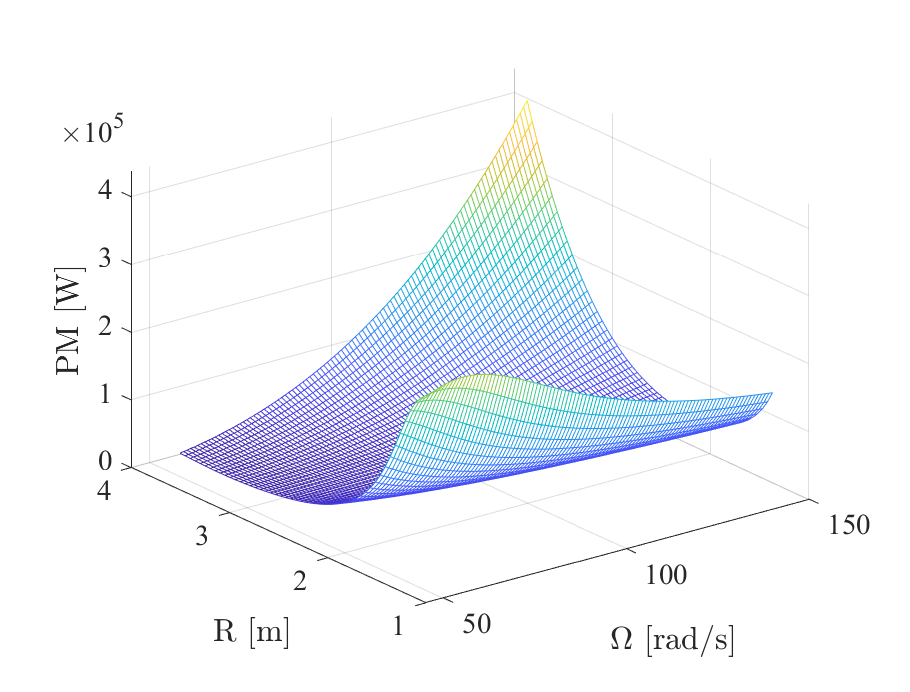
\includegraphics[width=80mm]{graficos/3d3d}
	\caption{Consumo de Potencia de la aeronave en función de la velocidad de giro del rotor y el radio del mismo.}
	\label{ORP}
\end{figure}
\begin{figure}
	\centering
	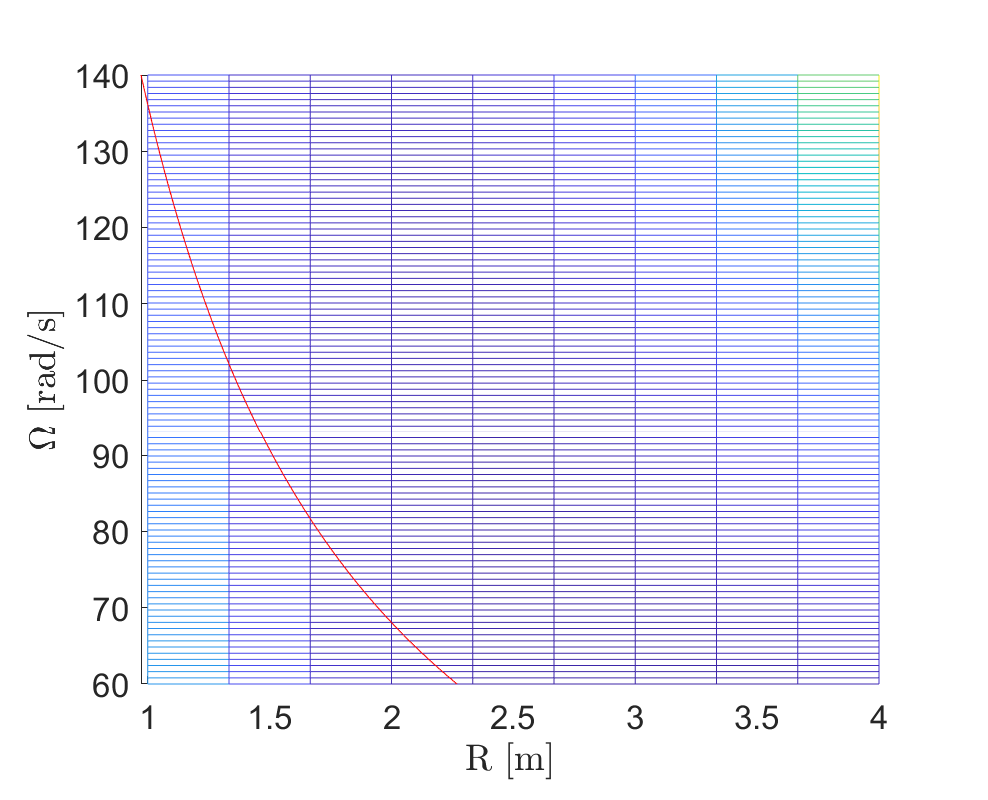
\includegraphics[width=80mm]{graficos/3d2d2}
	\caption{Consumo de Potencia de la aeronave en función de la velocidad de giro del rotor y el radio del mismo junto a la limitación de $\Omega$ a causa del $M_{crit}$ (0,4).}
	\label{ORPM}
\end{figure}

La gráfica \ref{ORP} representa la superficie que da un valor de potencia de la aeronave para cada $\Omega$ y R del rotor. Con esto es posible observar los valores mínimos de potencia, lo que nos permite elegir unos valores de $\Omega$ y R que optimicen la potencia necesaria.
Sin embargo, al añadir la limitación del $M_{crit}$ las opciones de configuración disponibles se ven reducidas a aquellas que la cumplan. La gráfica \ref{ORPM} representa la superficie de la gráfica \ref{ORP} sobre el plano $\Omega$R y encima la anterior limitación.
Se observa claramente que los valores de potencia necesaria se reducen con la potencia y con el aumento de radio, por lo que en primera instancia el menor valor dado, quedando automáticamente definido el radio del rotor.
\begin{itemize}
	\item Velocidad de giro del rotor principal $\Omega$ = 60 $rad/s$
	\item Radio del rotor principal $R$ = 2.26 $m$
\end{itemize}

\section{Helicóptero Semilla}

Con este helicoptero semilla se pueden realizar unas primeras simulaciones de vuelo para comprobar si es válido y, en caso contrario, modificar el diseño para alcanzar unos resultados mejores.